%%%%%%%%%%%%%%%%%%%%%%%%%%%%%%%%%%%%%%%%
% Classe do documento
%%%%%%%%%%%%%%%%%%%%%%%%%%%%%%%%%%%%%%%%

% Nós usamos a classe "unb-cic".  Deixe apenas uma das linhas
% abaixo não-comentada, dependendo se você for do bacharelado ou
% da licenciatura.

%\documentclass[bacharelado]{unb-cic}
\documentclass[licenciatura]{unb-cic}


%%%%%%%%%%%%%%%%%%%%%%%%%%%%%%%%%%%%%%%%
% Pacotes importados
%%%%%%%%%%%%%%%%%%%%%%%%%%%%%%%%%%%%%%%%

\usepackage[brazil,american]{babel}
\usepackage[T1]{fontenc}
\usepackage{indentfirst}
\usepackage{natbib}
\usepackage{xcolor,graphicx,url}
\usepackage[utf8]{inputenc}
\usepackage{hyperref}
\usepackage{acronym}
\usepackage{listings}
\usepackage{color}


\definecolor{dkgreen}{rgb}{0,0.6,0}
\definecolor{gray}{rgb}{0.5,0.5,0.5}
\definecolor{mauve}{rgb}{0.58,0,0.82}



\lstset{frame=tb,
	language=Java,
	aboveskip=3mm,
	belowskip=3mm,
	showstringspaces=false,
	columns=flexible,
	basicstyle={\small\ttfamily},
	numbers=none,
	numberstyle=\tiny\color{gray},
	keywordstyle=\color{blue},
	commentstyle=\color{dkgreen},
	stringstyle=\color{mauve},
	breaklines=true,
	breakatwhitespace=true,
	tabsize=3
}


%%%%%%%%%%%%%%%%%%%%%%%%%%%%%%%%%%%%%%%%
% Cores dos links
%%%%%%%%%%%%%%%%%%%%%%%%%%%%%%%%%%%%%%%%

% Veja o arquivos cores.tex se quiser ver que outras cores estão
% pré-definidas.  Utilizando o comando \hypersetup abaixo nós
% evitamos aquelas caixas vermelhas feias em volta dos links.

\input{cores}
\hypersetup{
  colorlinks=true,
  linkcolor=DarkScarletRed,
  citecolor=DarkScarletRed,
  filecolor=DarkScarletRed,
  urlcolor= DarkScarletRed
}



%%%%%%%%%%%%%%%%%%%%%%%%%%%%%%%%%%%%%%%%
% Informações sobre a monografia
%%%%%%%%%%%%%%%%%%%%%%%%%%%%%%%%%%%%%%%%

\title{Análise estática para detectar a evoulução da linguagem java em projetos open source}

\orientador{\prof \dr Rodrigo Bonifácio de Almeida}{CIC/UnB}
%\coorientador[a]{\prof[a] \dr[a] Coorientadora}{MAT/UnB}
\coordenador{\prof \dr Wilson Henrique Veneziano}{CIC/UnB}
\diamesano{31}{março}{2015}

\membrobanca{\prof \dr Genaina Nunes Rodriges}{CIC/UnB}
\membrobanca{\prof \dr Edson Alves}{CIC/UnB}

\autor{Thiago Gomes}{Cavalcanti}
\coautor{Vinícius Correa}{de Almeida}

\CDU{004.4}

\palavraschave{análise estática, evolução, evolução de linguagens de programação linguagens,language design, software engeneering, language evolution, refactoring, java}
\keywords{static analysis,language design, software engeneering, language evolution, refactoring, java}





%%%%%%%%%%%%%%%%%%%%%%%%%%%%%%%%%%%%%%%%
% Texto
%%%%%%%%%%%%%%%%%%%%%%%%%%%%%%%%%%%%%%%%
%\makeglossaries
\begin{document}
  \maketitle
  \pretextual

  \begin{dedicatoria}
	  Dedicamos este trabalho a nossa família e ao departamento de Ciência da Computação da UnB. Que este seja apenas uma ideia inicial para que outros alunos possam ajudar a enriquecer ainda mais este projeto para que a Universidade de Brasília tenha sua própria ferramenta de análise de código e que sirva de modelo para outras Universidades.

  \end{dedicatoria}

  \begin{agradecimentos}
	Com imensa dificuldade de agradecer a tantas pessoas que de certo modo nos ajudaram nessa conquista, hora em momentos calmos hora apreensivos. Em especial a toda nossa família por dar todo suporte necessário para que pudessemos concluir essa etapa em nossas vidas, também aluna Daniela Angellos pelo seu desdobramento e conhecimento para nos ajudar a criar essa ferramenta.\\
Em especial ao professor dr. Rodrigo Bonifácio que nos inseriu nesse imenso mundo da Engenharia de Software, hora apresentando um problemática hora ajundando a resolver barreiras as quais não conseguimos sozinhos.\\
E ainda a UnB por todo seu corpo docente que sem este essa jornada não seria concluida com excelência, em especial aoprofessor dr. Edson Alves da Costa Júnior por se deslocar da UnB-Gama para nos ajudar.\\

  \end{agradecimentos}

  \selectlanguage{brazil}
  \begin{resumo}
	Atualmente encontrar trechos de código específicos tem sido de grande importância para Utilizar linguagem de programa\c{c}\~{a}o como objeto de pesquisa \'{e} uma tarefa desafiadora e complexa quer seja para minerar informa\c{c}\~{o}es quer seja para refatorar, dada a complexidade de manipula\c{c}\~{a}o de uma linguagem de programa\c{c}\~{a}o. Entretanto existe um segmento da engenharia de \textit{software} que recomenda tratar este modelo de \textit{software} como qualquer outro onde este \'{e} denominado \textit{Grammarware}. 

Partindo deste segmento, este trabalho de conclus\~{a}o manipula c\'{o}digo fonte da linguagem Java para detectar constru\c{c}\~{o}es ultrapassadas. O principal objetivo deste trabalho foi tornar transparente a manipula\c{c}\~{a}o da linguagem Java para que fosse um simples \textit{input} como em qualquer outro \textit{software}. E isso mais f\'{a}cil adotar esta ferramenta para checar se a linguagem em que um software qualquer est\'{a} sendo desenvolvido utiliza sempre caracter\'{i}sticas atuais durante o desenvolvimento.

Desta forma o analisador est\'{a}tico que este trabalho proporcionou \'{e} capaz de pesquisar constru\c{c}\~{o}es espec\'{i}ficas da linguagem Java que podem ser facilmente determinadas por qualquer desenvolvedor independente da experi\^{e}cia na manipula\c{c}\~{a}o dos artefatos de uma linguagem de programa\c{c}\~{a}o.

Para a extra\c{c}\~{a}o dos dados este trabalho teve com principal preocupa\c{c}\~{a}o desacoplar a extra\c{c}\~{a}o da an\'{a}lise de c\'{o}digo para que os dados minerados possam ser salvos em qualquer estrutura de dado que pode ser desde um simples arquivo~\acs{CSV} at\'{e} um banco de dados.


  \end{resumo}


  \selectlanguage{american}
  \begin{abstract}
  	Use programming language like a research subject is a challenge and complex task either to mine information or to refactor, given the complexity of handling a programming language. However there is a segment of software engineering which recommends treating this model software like any other where this is called Grammarware.

From this segment, this final project handles source code of the Java language to detect outdated buildings. The main objective was to provide transparency in the handling of the Java language to make it a simple input as any other software. And easier to adopt this tool to check whether the language in which any software is being developed always uses current characteristics during development.

Thus the static analyzer that this work provided it is able to search for specific constructs of the Java language that can be easily determined by any independent developer of experience in handling the artifacts of a programming language.

For the extraction of data this work was with main concern to separate the extraction of code analysis and the mined data can be saved to any data structure that can be anything from a single file~\acs{CSV} accessible to a database.


%Search to specific code has been very important from update to a more actual or efficient and with the projetc has every the least release of a language at this work Java.

%Therefore the main goal of this project is develop a static analysis with objective to find specifics constructions of Java language, where this constructions can be older code or a update a block to another better such as foreach for a lambda expression. After find this code the place in source code is saved to write a output file for future evaluation and decide if this will be updated or not.

%With focus in a flexibility the project the party responsible for visitors that find source code previously determined is the highest flexible that make easy in any time the developer create their own visitor and insert in the system without impacts in architecture. The output reports are flexible and automatics that provide in any time a possibility of chance the actuals ~\acs{CSV} files to another form such as database.
  \end{abstract}
  
  
  \selectlanguage{brazil}


  \tableofcontents
  \listoffigures
  \listoftables
  
  
  %\newpage
  \addcontentsline{toc}{chapter}{Lista de Abreviaturas}
  \chapter*{Lista de abreviaturas}
  \begin{acronym}
\acro{LOC}{Linhas de Código}%
\acro{AST}{Árvore de sintaxe abstrata}%
\acro{IDE}{Ambiente de Desenvolvimento Integrado}
\acro{JDBC}{Java Database Connectivity}
\acro{JDK}{Java Development Kit}
\acro{AWT}{Abstract Window Toolkit}
\acro{RMI}{Invocação de Método Remoto}
\acro{API}{Aplicações de Programação Interfaces}
\acro{JNI}{Java Native Interface}
\acro{GUI}{Interface Gráfica do Usuário}
\acro{JDT}{Java Development Tools}
\acro{ACDP}{Java Platform Debugger Architecture}
\acro{JCP}{Java Community Process}
\acro{EFL}{Enhanced for loop}
\acro{AIC}{Annonymous Inner Class}
\acro{DI}{Dependency Injection}
\acro{IoC}{Inversion of Control}
\acro{CSV}{Comma separated values}


\end{acronym}
  
%  \newpage
 % \addcontentsline{toc}{chapter}{List of Abbreviations}
 % \chapter*{List of Abbreviations}
  

  \textual
 
  \include{capitulos/capitulo1_Introducao}
\include{capitulos/capitulo1_historia_da_linguagem}
\section {Aspectos evolutivos da liguagem Java}
		\subsection {Java 2}
			A primeira versão do Java Security, disponível no JDK 1.1 \cite{JDK1.1}, contém um subconjunto dessa funcionalidade, incluindo APIs para:
		  \begin{itemize}
			  \item Assinaturas Digitais: Algoritmos de assinatura digital, como DSA ou MD5 com RSA. A funcionalidade inclui a geração de chaves público/privado , bem como assinatura e verificação de dados digitais.
			  \item Gerenciamento de Chaves: Um conjunto de abstrações para o gerenciamento de ''diretores'' (entidades como usuários individuais ou grupos), suas chaves, e os seus certificados. Ele permite que aplicativos para projetar seu próprio sistema de gerenciamento de chaves, e para interoperar com outros sistemas em alto nível.
			  \item Lista de controle de acesso: Um conjunto de abstrações para o gerenciamento de ''diretores'' e suas permissões de acesso.
			  \item A obtenção de um objeto de assinatura: 
			  
\begin{lstlisting}
import java.security.Signature;
import java.security.NoSuchAlgorithmException;
	
public class SignFile {
	Signature signature;
		
	private void init(String algorithm) throws NoSuchAlgorithmException{
		signature = Signature.getSignature(algorithm);
    }
}
\end{lstlisting}
			  
			  \item Em versões anteriores, Java suportava apenas {\it top-level} classes, que devem ser membros de pacotes. Na versão 1.1, o programador Java pode agora definir classes internas como membros de outras classes \cite{bracha1998gj}, localmente dentro de um bloco de instruções, ou (anonimamente) dentro de uma expressão.
		  
\begin{lstlisting}
public class FixedStack {
	...
	 public java.util.Enumeration elements() {
	     return new FixedStack$Enumerator(this);
	 }
}
		
class FixedStack$Enumerator implements java.util.Enumeration {
	private FixedStack this$0;
	
	FixedStack$Enumerator(FixedStack this$0) {
		this.this$0 = this$0;
		this.count = this$0.top;
	 }
			
	int count;
	public boolean hasMoreElements() {
		return count > 0;
	}
		
	public Object nextElement() {
		if (count == 0)
			throw new NoSuchElementException("FixedStack");
		
		return this$0.array[--count];
	}
}
\end{lstlisting}
			
			\clearpage
			\item Para escrever um objeto remoto (RMI), você escrever uma classe que implementa uma ou mais interfaces remotas. 
			
\begin{lstlisting}
package examples.hello;
public interface Hello extends java.rmi.Remote {
	String sayHello() throws java.rmi.RemoteException;
}
\end{lstlisting}
	 
\item HelloImpl.java
\begin{lstlisting}
package examples.hello;

import java.rmi.;
import java.rmi.server.UnicastRemoteObject;

public class HelloImpl extends UnicastRemoteObject implements Hello{
	private String name;
	
	public HelloImpl(String s) throws RemoteException {
		super();
		name = s;
	}
	
	public String sayHello() throws RemoteException {
		return  "Hello World!";
	}
	
	public static void main(String args[]){
	
		System.setSecurityManager(new RMISecurityManager());
	
		try {
			HelloImpl obj = new HelloImpl("HelloServer");
			Naming.rebind("//myhost/HelloServer", obj);
			System.out.println("HelloServer bound in registry");
		} catch (Exception e) {
			System.out.println("HelloImpl err: " + e.getMessage());
			e.printStackTrace();
		}
	}
}
\end{lstlisting}
		\end{itemize}


	\clearpage
	\subsection {Java 4}
	  \begin{itemize}
		  \item {\it Assertion Facility} \cite{JSE8_Enhancements}. As {\it assertions} são expressões booleanas que o programador acredita ser verdade sobre o estado de um programa de computador. Por exemplo, depois de ordenar uma lista o programador pode afirmar que a lista está em ordem crescente. Avaliando as afirmações em tempo de execução para confirmar a sua validade é uma das ferramentas mais poderosas para melhorar a qualidade do código, uma vez que rapidamente se descobre equívocos do programador sobre o comportamento de um programa.
	  \end{itemize}
	
	\subsection {Java 5}
	  \begin{itemize}
		  \item {\it Generics}\cite{JSE8_Enhancements, OracleGenerics,Parnin:2011:JGA:1985441.1985446}. Este novo recurso para o sistema de tipo permite que um tipo ou método operar em objetos de vários tipos, proporcionando em tempo de compilação tipo de segurança. Acrescenta em tempo de compilação um tipo de segurança para as {\it collections} e elimina o trabalho penoso de {\it casting}. Um exemplo do uso de {\it colletions} e {\it generics} respectivamente:
\begin{lstlisting}
static void expurgate(Collection c) {
	for (Iterator i = c.iterator(); i.hasNext(); )
		if (((String) i.next()).length() == 4)
			i.remove();
	}
	
static void expurgate(Collection<String> c) {
	for (Iterator<String> i = c.iterator(); i.hasNext(); )
		if (i.next().length() == 4)
			i.remove();
}
\end{lstlisting}
		  
		\item {\it For-Each Loop}. Esta nova estrutura de linguagem elimina o trabalho e erro de propensão de iteradores e variáveis de índice quando a iteração ocorre sobre coleções e arrays. Como a construção evoluiu com o advento dessa nova estrutura:
	
\begin{lstlisting}
void cancelAll(Collection<TimerTask> c) {
	for (Iterator<TimerTask> i = c.iterator(); i.hasNext(); )
	   i.next().cancel();
}
	
void cancelAll(Collection<TimerTask> c) {
	for (TimerTask t : c)
		t.cancel();
}
\end{lstlisting}
	  
	  \clearpage
	  \item {\it Varargs}. Esta nova estrutura tende a eliminar a necessidade de passagem manual de listas de argumentos em um array ao invocar métodos que aceitam de um comprimento variável de uma lista de argumentos. Nas versões anteriores, um método levava um número arbitrário de valores necessários a  criar uma matriz e colocar os valores para a matriz antes de chamar o método.


\begin{lstlisting}
public class Test {
	public static void main(String[] args) {
	  int passed = 0;
	  int failed = 0;
	  for (String className : args) {
	      try {
	          Class c = Class.forName(className);
	          c.getMethod("test").invoke(c.newInstance());
	          passed++;
	      } catch (Exception ex) {
	          System.out.printf("%s failed: %s%n", className, ex);
	          failed++;
	      }
	  }
	  System.out.printf("passed=%d; failed=%d%n", passed, failed);
	}
}
\end{lstlisting}
 
	  \item {\it Autoboxing/Unboxing}. Esta nova estrutura elimina o trabalho de conversão manual entre tipos primitivos (como {\it int}) e os tipos de classes {\it wrapper}
  \end{itemize}
  
  
  
	\subsection {Java 6}
		Não ocorram mudanças ou introdução de novas estruturas na linguagem Java \cite{JSE8_Enhancements}.
	
	\subsection {Java 7}
		\begin{itemize}
		  \item {\it Multi Catch} e lançamento de exceções com melhora na verificação de tipos. Um único bloco {\it catch} poderá lidar com mais de um tipo de exceção. Além disso, o compilador executa a análise mais precisa das exceções. Isso permite que o programador especifique tipos de exceção mais específicos na cláusula de uma declaração método. Um exemplo de como era as estruturas que usavam {\it cacths} e com a introdução de {\it multi catch} com o Java 7 \cite{JSE7}, respectivamente.
  

\begin{lstlisting}
catch (IOException ex) {
	logger.log(ex);
	throw ex;
}catch (SQLException ex) {
	logger.log(ex);
	throw ex;
}
\end{lstlisting}
\clearpage
\begin{lstlisting}
catch (IOException|SQLException ex) {
	logger.log(ex);
	throw ex;
}
\end{lstlisting}


 \item O {\it try-with-resouces}. A declaração {\it try-with-resouces} é uma instrução {\it try} que declara um ou mais recursos. Um recurso é um objeto que deve ser fechada após o programa terminar com ele. Essa declaração garante que cada recurso é fechada no final da declaração.
	 
\begin{lstlisting}

public static void writeToFileZipFileContents(
			String zipFileName, String outputFileName) throws java.io.IOException {
	
	java.nio.charset.Charset charset = java.nio.charset.StandardCharsets.US_ASCII;
	java.nio.file.Path outputFilePath = java.nio.file.Paths.get(outputFileName);
	
	try(
		 java.util.zip.ZipFile zf = new java.util.zip.ZipFile(zipFileName);
		 java.io.BufferedWriter writer = java.nio.file.Files.newBufferedWriter(outputFilePath, charset)
	){
	
		for (java.util.Enumeration entries = zf.entries(); entries.hasMoreElements();) {
			 String newLine = System.getProperty("line.separator");
			 String zipEntryName = ((java.util.zip.ZipEntry)entries.nextElement()).getName() + newLine;
			 writer.write(zipEntryName, 0, zipEntryName.length());
		 }
	}
}

\end{lstlisting}
		  
		  \clearpage
		  \item Inferência de tipos para criação de instâncias em {\it generics}\cite{OracleGenerics}\cite{Bracha:1998:MFS:286942.286957}\cite{Parnin:2011:JGA:1985441.1985446}. Com o Java 7 pode-se substituir os argumentos de tipo necessários para invocar o construtor de uma classe genérica com um conjunto vazio de parâmetros de tipo (<>), desde que o compilador infira os argumentos de tipo a partir do contexto. Este par de colchetes angulares é informalmente chamado de diamante.
  
  

\begin{lstlisting}
Map<String, List<String>> myMap = new HashMap<String, List<String>>();
Map<String, List<String>> myMap = new HashMap<>();
	
List<String> list = new ArrayList<>();
list.add("A");

list.addAll(new ArrayList<>());
	
class MyClass<X> {
	<T> MyClass(T t) {
	...
	}
}
\end{lstlisting}
	 
	  \end{itemize}
	  
	  
	\subsection{Java 8}
	  \begin{itemize}
		  \item Melhoria na inferência de tipos. O compilador Java aproveita digitação para inferir os parâmetros de tipo de uma invocação de método genérica. O tipo de destino de uma expressão é o tipo de dados que o compilador Java espera, dependendo de onde a expressão aparece. Por exemplo, pode-se usar o tipo de destino de uma instrução de atribuição para o tipo de inferência em Java 7. No entanto, em Java 8, pode-se usar o tipo de destino para a inferência de tipos em mais contextos. O exemplo mais proeminente está usando tipos de destino de um método de invocação para inferir os tipos de dados dos seus argumentos.

\begin{lstlisting}
	List<String> stringList = new ArrayList<>();
	stringList.add("A");
	stringList.addAll(Arrays.asList());
\end{lstlisting}
		  
		  
		  \item Expressões lambda. Permitem encapsular uma única unidade de comportamento e passá-lo para outro código. Pode-se usar uma expressãos lambda, se quiser uma determinada ação executada em cada elemento de uma {\it collection}, quando o processo for concluído, ou quando um processo encontra um erro. \cite{JSE7} \\
	  \end{itemize}

\clearpage
\begin{lstlisting}
public class Calculator {
	
	interface IntegerMath {
		int operation(int a, int b);   
	}

	public int operateBinary(int a, int b, IntegerMath op) {
		return op.operation(a, b);
	}

	public static void main(String... args) {

		Calculator myApp = new Calculator();
		IntegerMath addition = (a, b) -> a + b;
		IntegerMath subtraction = (a, b) -> a - b;
		System.out.println("40 + 2 = " + myApp.operateBinary(40, 2, addition));
		System.out.println("20 - 10 = " + myApp.operateBinary(20, 10, subtraction));    
		
	}
}
\end{lstlisting}
\chapter{Problema a ser Atacado}
\section{Problematização}

Nos últimos anos sistemas computacionais ganharam cada vez mais espaço no mercado o que acarretou na dedicação de profissionais para manter a qualidade elevada tanto no desenvolvimento como na manutenção destes a fim de proporcionar tanto a multiplataforma quanto que qualquer equipe seja capaz de desenvolvem em qualquer local a qualquer tempo.\\

Com isso a produção de software tornou-se uma tarefa desafiadora de altíssima complexidade que pode acarretar no aumento da possibilidade de surgimento de problemas. Outro fator de grande relevância é que cada vez mais o bom desempenho do software depende da capacidade e qualificação dos profissionais que compoẽm a equipe de desenvolvimento. Um desses problemas é manter o desenvolvimento com partes ultrapassadas de uma linguagem o que torna um sistema obsoleto e com a chance de conter bugs e vulnerabilidades que podem comprometer a segurança de todo o sistema.\\


A atuação de equipes que desenvolvem utilizando códigos obsoletos continua sendo um grande problema no desenvolvimento de software ao longo de suas releases, mesmo com a evolução da linguagem. Códigos mais atuais tornam-se cada vez mais necessário pois evitam, corrigem falhas e vulnerabilidades além do mesmo tornar-se mais atual. Tais códigos não evoluem podem ser por falta de suporte da IDE, por falta conhecimento da equipe de desenvolvedora ou pelo simples fato de não possuir uma analisador estático que aborde estas construções lançadas nas novas versões das linguagens, especificamente java.\\


Após toda release uma linguagem demora um certo tempo de maturação para que comunidade de desenvolvedores adote novas características lançadas ou simplesmente não a utilizem, porém java possui uma filosofia de manter suporte a todos legado já desenvolvido por questão de portabilidade o que beneficia tanto IDE's quanto equipes a não ter a necessidade de se atualizarem para as ultimas versões da linguagem o que torna a construção de software com uma linguagem ultrapassada confortável porém existe a possibilidade do software possuir vulnerabilidades.\\

Um bom exemplo a ser lembrado é FORTRAN quando adicionou orientação objetos em sua release \textbf{XX} forçando a evoulução de seus compiladores os quais não forneciam mais suporte a versões anteriores conforme relata Jeffrey L. Overbey e Ralph E. Johnson em \cite{Overbey:2009:RLR:1639949.1640127}, que como consequência forçou toda comunidade desenvolvedora a se atualizar. E ainda havia a possiblidade de certos trechos de código sofrer um refectoring em tempo de compilação por um código mais atual e equivalente.\\

A processo de utilizar um analisador estático em um projeto antes de sua compilação pode vir a impactar na melhora da confiança do software pois pode detectar vulnerabilidades de maneira prematura além de reduzir o retrabalho caso estas não fossem detectadas. Tais vulnerabilidades são falhas que podem vir a ser exploradas por usuários maliciosos, estes podem desde obter acesso ao sistema, manipular dados ou até mesmo tornar todo serviço indisponível. Neste trabalho a criação de um analisador estático terá o intuito de pesquisar trechos de código ultrapassado.\\

A implementação de refectoring na grande parte das modernas IDEs mantem suporte para um simples conjunto de código onde o comportamento é intuitivo e fácil de ser analisado,  quando características avançadas de uma linguagem com o java são usados descrever precisamente o comportamento de tarefas é de extrema complexidade além da implementação do refectoring ficar complexa e de difícil entendimento segundo Max Schäfer e Oege de Moor em \cite{Schaefer:2010:SIR:1932682.1869485}. Modernas IDEs como ecplise realizam complexos refectoring através da técnica de microrefectoring que nada mais é que a divisão de um bloco de código complexo em pequenas partes para tentar encontrar códigos mais intuitivos a serem modificados.\\

O analisador estático proposto nesse trabalho tem o objeto de identificar construções ultrapassadas e porções de código congelados que são utilizadas ao logo do desenvolvimento do software verificando o histórico do lançamento das releases de software livres desenvolvidos em especialmente usando a linguagem java. Ainda caberá ao desenvolvedor tomar a decisão caso existam construções ultrapassadas nas releases se adotará o refectoring ou manterá o código congelado expondo o mesmo a usuários maliciosos.\\







  \chapter{Java}
\section {Historia da linguagem}

No começo da decada de 90 um pequeno grupo de engenheros da Oracle chamados de ''Green Team'' acreditava que a próxima onde de na area da computação seria a união de equipamentos eletroeletrônicos com os computadores. O ''Green Team'' liderado por James Gosling, demonstraram que a linguagem de programaçao Java, que foi desenvolvida pela equipe e originalmente era chamado de Oak, foi desenvolvida para dispositivos de entretenimento como aparelhos de tv a cabo, porem não foi bem aceita no meio. Em 1995 com a massificação da Internet foi quando a linguagem Java teve sua primeira grande aplicação o navegador Netscape.\\

Java é uma linguagem de programação de propósito geral orientada a objetos, concebida especificadademente para ter poucas dependencias de implementação que isso acarreta que uma vez que a aplicação fora desenvolvida ela poderá ser executada em qualquer lugar.\\

Na sua primeira versão chamada de Java 1 (JDK* 1.0.2) onde introduziram oito pacotes básicos do java como: java.lang, java.io, java.util, java.net, java.awt, java.awt.image, java.awt.peer e java.applet. Foi usado para o desenvolvimento de ferramentas populares na epoca como o Netscape 3.0 e o Internet Explorer 3.0. \\

Sua segunda versão foi o JDK* 1.1 onde trouxe ganhos em funcionalidades, desempenho e qualidade. Novas aplicações tambem surgiram como : JavaBeans, aprimoramento do AWT*, novas funcionalidades como o JDBC*, acesso remoto ao objeto (RMI*) e suporte ao padrão Unicode 2.0.\\

Na terceira versão Java 2 (JDK* 1.2) ofereceu melhorias significativas no desempenho, um novo modelo de segurança, flexível e um conjunto completo de aplicações de programação interfaces (APIs). Os novos recursos da plataforma Java 2 incluiram: 
\begin{itemize}
  \item O modelo de "sandbox"  foi ampliado para dar aos desenvolvedores, usuários e administradores de sistema a opção de especificar e gerenciar um conjunto de políticas de segurança flexíveis que governam as ações de uma aplicação ou applet que pode ou não ser executada.
  \item Suporte nativo a thread para o ambiente operacional Solaris. Compressão de memória para classes carregadas. Alocação de memória com mais desempenho e melhor para a coleta de lixo. Arquitetura de máquina virtual conectável para outras máquinas virtuais, incluindo a Java HotSpot VMNew. Just in Time (JIT*). Java Native Interface (JNI*) de conversão.
  \item O conjunto de componentes de projeto, GUI (Swing). API Java 2D que fornece novos recursos gráficos 2D e AWT*, bem como suporte para impressão. O Java {\it look and fell} de interface. Uma nova API de acessibilidade.
  \item Framework de entrada de caracteres (suporte a japonês, chinês e coreano). Complexo de saída usando a API* do Java 2D para fornecer um {\it display} bi-direcional, de alta qualidade de japonês, árabe, hebraico e outras línguas de caracteres.
  \item Java Plug-in para navegadores da Web, incluída na plataforma Java 2, fornecendo um tempo de execução totalmente compatível com a máquina virtual Java amplamente implantadas em navegadores.
  \item Invocação das operações ou serviços de rede remoto. Totalmente compatível com Java ORB e incluído no tempo de execução.
  \item JDBC que fornece um acesso mais fácil aos dados para consultas mais flexíveis. Melhor desempenho e estabilidade são promovidos por cursores de rolagem e suporte para SQL3 de tipos.\\
\end{itemize}

Em 8 de maio de 2000 foi anunciado o Java 2 versão 1.3 que trouxe ganho de desempenho em relação a primeira versão da JS2E* de cerca de 40\%  no tempo de {\it  start-up} e de 20\%. Tambem trouxe novas funcionaliadades como: 

\begin{itemize}
  \item O Java HotSpot VM* de cliente e suas bibliotecas atentando ao desempenho ao fazer o J2SE* versão 1.3 a {\it realease} o mais rápido até à data.
  \item Novos recursos, como o {\it caching applet} e instalação do pacote opcional Java através da tecnologia Java {\it  Plug-in} para aumentar a velocidade e a flexibilidade com que os {\it applets} e aplicativos baseados na tecnologia Java pode ser implantado. Java {\it  Plug-in} tecnologia é um componente do ambiente de execução Java 2, Standard Edition v 1.3 que permite Java {\it applets} e aplicativos para a execução.
  \item O novo suporte para RSA* assinatura eletrônica, gerenciamento de confiança dinâmico, certificados X.509, e verificação de arquivos o que significa o aumento das possibilidades que os desenvolvedores tem para proteger dados eletrônicos.
  \item Uma série de novos recursos e ferramentas de desenvolvimento da tecnologia J2SE* versão 1.3 que permite o desenvolvimento mais fácil e rápido de aplicações baseadas na tecnologia {\it web} ou Java {\it  standalone} de alto desempenho.
  \item A adição de RMI / IIOP* e o Jndi (JNDI*) para a versão 1.3, melhora na interoperabilidade J2SE*. RMI / IIOP* melhora a conectividade com sistemas de {\it  back-end} que suportam CORBA*. JNDI fornece acesso aos diretórios que suportam o populares LDAP* Lightweight Directory Access Protocol, entre outros.\\
\end{itemize}

No ano de 2000 no dia 6 de Fevereiro, foi lançado a J2SE* versão 1.4. Com a versão 1.4, as empresas puderam usar a tecnologia Java para desenvolver aplicativos de negócios mais exigentes e com menos esforço e em menos tempo. As novas funcionalidades como a nova I/O* e suporte a 64 bits. A J2SE* se tornou plataforma ideal para a mineração em grande escala de dados, inteligência de negócios, engenharia e científicos. A versão 1.4 forneceu suporte aprimorado para tecnologias padrões da indústria, tais como SSL*, LDAP* e CORBA* a fim de garantir a operacionalidade em plataformas heterogêneas, sistemas e ambientes. Com o apoio embutido para XML*, a autenticação avançada, e um conjunto completo de serviços de segurança, está versão forneceu base para padrões de aplicações Web e serviços interoperáveis. O J2SE* avançou o desenvolvimento de aplicativos de cliente com novos controles de GUI, acelerou Java 2D, a performance gráfica, internacionalização e localização expandida de apoio, novas opções de implantação e suporte expandido para o até então Windows XP.\\

Com a chegada da JSE2* versão 1.5 (Java 5.0) em 6 de ferevereiro de 2002, impulsionou benefícios extensivos para desenvolvedores, incluindo a facilidade de uso, desempenho global e escalabilidade, monitoramento do sistema e gestão e desenvolvimento. O Java 5 foi derivado do trabalho de 15 componentes Java Specification Requests (JSRs) englobando recursos avançados para a linguagem e plataforma. Os líderes da indústria na época que participam no grupo de peritos J2SE 5.0 incluiram: Apache Software Foundation, Apple Computer, BEA Systems, Borland Software Corporation, Cisco Systems, Fujitsu Limited, HP, IBM, Macromedia, Nokia Corporation, Oracle, SAP AG, SAS Institute, SavaJe Technologies e Sun Microsystems.

Novas funcionalidades foram implementadas como:

\begin{itemize}
  \item Facilidade de desenvolvimento: os programadores da linguagem Java pode ser mais eficiente e produtivos com os recursos de linguagem Java 5 que permitiram a codificação mais segura. Nesta versão surgiu {\it Generics}, tipos enumerados, metadados e autoboxing de tipos primitivos permitindo assim uma fácil e rápida codificação.
  \item Monitoramento e gestão: Um foco chave para a nova versão da plataforma, a aplicativos baseados na tecnologia Java {\it Virtual Machine} que passou a ser monitorado e gerenciado com o {\it built-in} de suporte para Java {\it Management Extensions}. Isso ajudou a garantir que seus funcionários, sistemas de parceiros do cliente permanecessem em funcionamento por mais tempo. Suporte para sistemas de gestão empresarial baseados em SNMP* também é viável.
  \item Um olhar novo aplicativo, mais moderna, baseada na tecnologia Java padrão e proporciona uma sensação GUI para aplicativos baseados na tecnologia Java. A J2SE* 5.0 teve suporte completo a internacionalização e também possuindo suporte para aceleração de hardware por meio da API OpenGL* e tambem para o sistema operacional Solaris e sistemas operacionais da distribuição Linux.
  \item Maior desempenho e escalabilidade: A nova versão incluiu melhorias de desempenho, tais como menor tempo de inicialização, um menor consumo de memória e JVM* auto ajustável para gerar maior desempenho geral do aplicativo e desenvolvimento em J2SE 5.0 em relação às versões anteriores.\\
\end{itemize}

Java 1.6 (Java 6) foi divulgado em 11 de dezembro de 2006. Tornou o desenvolvimento mais fácil, mais rápido e mais eficiente em termos de custos e ofereceu funcionalidades para serviços web, suporte linguagem dinâmica, diagnósticos e aplicações desktop. Com a chegada dessa nova versão do Java houve combinação com o NetBeans IDE 5.5 fornecendo aos desenvolvedores uma estrutura confiável, de codigo aberto e compatível, de alta performance para entregar aplicativos baseados na tecnologia Java mais rápido e mais fácil do que nunca. O NetBeans IDE* fornece uma fonte aberta e de alto desempenho, modular, extensível, multi-plataforma Java IDE* para acelerar o desenvolvimento de aplicações baseadas em software e serviços {\it web}.
Novas funcionalidades foram implementadas como:

\begin{itemize}
  \item O Java 1.6 ajudou a acelerar a inovação para o desenvolvedor, aplicativos de colaboração {\it online} e baseadas na {\it web}, incluindo um novo quadro de desenvolvedores APIs para permitir a mistura da tecnologia Java com linguagens de tipagem dinâmica, tais como PHP, Python, Ruby e tecnologia JavaScript. A Sun também criou uma coleção de mecanismos de script e pré-configurado o motor JavaScript Rhino na plataforma Java. Além disso, o software inclui uma pilha completa de clientes de serviços web e suporta as mais recentes especificações de serviços {\it web}, como JAX-WS 2.0*, JAXB 2.0*, STAX* e JAXP.*
  \item A plataforma Java 1.6 forneceu ferramentas expandidas para o diagnóstico, gestão e monitoramento de aplicações e também inclui suporte para o novo NetBeans Profiler 5.5 para Solaris DTrace e, uma estrutura de rastreamento dinâmico abrangente que está incluído no sistema operacional Solaris 10. Além disso, o software Java SE 6 aumenta ainda mais a facilidade de desenvolvimento com atualizações de interface ferramenta para o Java Virtual Machine (JVM) e o Java Platform Debugger Architecture (ACDP)*.
\end{itemize}

Java 7 foi lançado no dia 28 de julho de 2011. Essa versão foi resultado do desenvolvimento de toda a indústria envolvendo uma revisão de codigo aberto e extensa colaboração entre os engenheiros da {\it Oracle} e membros do ecossistema Java em todo o mundo através da comunidade {\it OpenJDK} e do {\it Java Community Process} (JCP)*. Compatibilidade com versões anteriores de Java 7 com versões anteriores da plataforma a fim de preservar os conjuntos de habilidades dos desenvolvedores de software Java e proteger os investimentos em tecnologia Java.

Com essa versão novas funcionalidades foram adicionadas:

\begin{itemize}
  \item As alterações de linguagem ajudaram a aumentar a produtividade do desenvolvedor e simplificar tarefas comuns de programação, reduzindo a quantidade de código necessário, esclarecendo sintaxe e tornar o código com mais legibilidade.
  \item Melhor suporte para linguagens dinâmicas incluindo: Ruby, Python e JavaScript, resultando em aumentos substanciais de desempenho no JVM*.
  \item Uma nova API* {\it multicore-ready} que permite aos desenvolvedores para se decompor mais facilmente problemas em tarefas que podem ser executadas em paralelo em números arbitrários de núcleos de processador.
  \item Uma interface de I/O* abrangente para trabalhar com sistemas de arquivos que podem acessar uma ampla gama de atributos de arquivos e oferecem mais informações quando ocorrem erros.
  \item Novos recursos de rede e de segurança. Suporte expandido para a internacionalização, incluindo suporte a Unicode 6.0. Versões atualizadas das bibliotecas padrão.\\
  \item
  \item
  \item
  \item
\end{itemize}



\\

\section {Aspectos evolutivos da liguagem Java}
\subsection {Java 1}
\subsection {Java 2}
\subsection {Java 3}
\subsection {Java 4}
\subsection {Java 5}
\subsection {Java 6}
\subsection {Java 7}
\subsection {Java 8}
 



								
  %\chapter{Fundamentação}
\section{Linguagem Java}
No começo da década de 90 um pequeno grupo de engenheiros da Oracle chamados de "\textit{Green Team}" acreditava que a próxima onde de na area da computação seria a união de equipamentos eletroeletrônicos com os computadores. O "\textit{Green Team}" liderado por James Gosling, demonstraram que a linguagem de programação Java, que foi desenvolvida pela equipe e originalmente era chamado de Oak, foi desenvolvida para dispositivos de entretenimento como aparelhos de tv a cabo, porem não foi bem aceita no meio. Em 1995 com a massificação da Internet, a linguagem Java teve sua primeira grande aplicação o navegador Netscape.

Java é uma linguagem de programação de propósito geral orientada a objetos, concebida especificadamente para ter poucas dependências de implementação que isso acarreta que uma vez que a aplicação fora desenvolvida ela poderá ser executada em qualquer ambiente computacional.

Na sua primeira versão chamada de Java 1 (\acs{JDK} 1.0.2) haviam oito pacotes básicos do java como: java.lang, java.io, java.util, java.net, java.awt, java.awt.image, java.awt.peer e java.applet. Foi usado para o desenvolvimento de ferramentas populares na época como o Netscape 3.0 e o Internet Explorer 3.0.

Sua segunda versão foi o \acs{JDK}1.1 \cite{JDK1.1} que trouxe ganhos em funcionalidades, desempenho e qualidade. Novas aplicações tambem surgiram como : JavaBeans, aprimoramento do \acs{AWT}, novas funcionalidades como o \acs{JDBC}, acesso remoto ao objeto \acs{RMI} e suporte ao padrão Unicode 2.0.\\

A terceira versão Java 2 (\acs{JDK} 1.2) ofereceu melhorias significativas no desempenho, um novo modelo de segurança, flexível e um conjunto completo de aplicações de programação interfaces \acs{API}'s. O modelo de "\textit{sandbox}" foi ampliado para dar aos desenvolvedores, usuários e administradores de sistema a opção de especificar e gerenciar um conjunto de políticas de segurança flexíveis que governam as ações de uma aplicação ou \textit{applet} que pode ou não ser executada. Foi introduzido o suporte nativo a \textit{thread} para o ambiente operacional Solaris e também a compressão de memória para classes carregadas. Alocação de memória com mais desempenho e melhor para a coleta de lixo. Arquitetura de máquina virtual conectável para outras máquinas virtuais, incluindo a \textit{Java HotSpot VMNew}. \textit{Java Native Interface }\acs{JNI} de conversão. O novo conjunto de componentes de projeto, \acs{GUI} (\textit{Swing}). \acs{API} Java 2D que fornece novos recursos gráficos 2D e \acs{AWT}, bem como suporte para impressão. Java \textit{plug-in} para navegadores da \textit{web}, incluída na plataforma Java 2, fornecendo um tempo de execução totalmente compatível com a máquina virtual Java amplamente implantadas em navegadores. A inclusão do \acs{JDBC} que fornece um acesso mais fácil aos dados para consultas mais flexíveis e trouxe melhor desempenho e estabilidade promovidos por cursores de rolagem e suporte para SQL3 de tipos.\\


Em 8 de Maio de 2000 foi anunciado o Java 2 versão 1.3 que trouxe ganho de desempenho em relação a primeira versão da JS2E de cerca de 40\%  no tempo de {\it  start-up}. O {\it Java HotSpot VM} de cliente e suas bibliotecas atentando ao desempenho ao fazer o J2SE versão 1.3 a {\it realease} o mais rápido até à data. Novos recursos, como o {\it caching applet} e instalação do pacote opcional Java através da tecnologia Java {\it  Plug-in} para aumentar a velocidade e a flexibilidade com que os {\it applets} e aplicativos baseados na tecnologia Java podem ser implantados. Java {\it  Plug-in} tecnologia é um componente do ambiente de execução Java 2 que permite Java {\it applets} e aplicativos para a execução. O novo suporte para \acs{RSA} assinatura eletrônica, gerenciamento de confiança dinâmico, certificados X.509, e verificação de arquivos o que significa aumento das possibilidades que os desenvolvedores tem para proteger dados eletrônicos. Uma série de novos recursos e ferramentas de desenvolvimento da tecnologia J2SE versão 1.3 que permite o desenvolvimento mais fácil e rápido de aplicações baseadas na tecnologia {\it web} ou Java {\it  standalone} de alto desempenho. A adição de RMI/IIOP e o JNDI para a versão 1.3, melhora na interoperabilidade J2SE. Melhora da conectividade com sistemas de {\it  back-end} que suportam CORBA. O novo suporte que o JNDI fornece acesso aos diretórios que suportam o populares LDAP Lightweight Directory Access Protocol, entre outros.\\


No ano de 2002 no dia 6 de Fevereiro, foi lançado a J2SE versão 1.4. Com a versão 1.4, as empresas puderam usar a tecnologia Java para desenvolver aplicativos de negócios mais exigentes e com menos esforço e em menos tempo. As novas funcionalidades como a nova I/O e suporte a 64 bits. A J2SE se tornou plataforma ideal para a mineração em grande escala de dados, inteligência de negócios, engenharia e científicos. A versão 1.4 forneceu suporte aprimorado para tecnologias padrões da indústria, tais como SSL, LDAP e CORBA a fim de garantir a operacionalidade em plataformas heterogêneas, sistemas e ambientes. Com o apoio embutido para XML, a autenticação avançada, e um conjunto completo de serviços de segurança, está versão forneceu base para padrões de aplicações Web e serviços interoperáveis. O J2SE avançou para o desenvolvimento de aplicativos de cliente com novos controles de GUI, acelerou Java 2D, a performance gráfica, internacionalização e localização expandida de apoio, novas opções de implantação e suporte expandido para o até então {\it Windows XP}.\\

Com a chegada da \acs{JSE2} versão 1.5 (Java 5.0) em 30 de Setembro de 2004, impulsionou benefícios extensivos para desenvolvedores, incluindo a facilidade de uso, desempenho global e escalabilidade, monitoramento do sistema e gestão e desenvolvimento. O Java 5 foi derivado do trabalho de 15 componentes Java Specification Requests (JSRs) englobando recursos avançados para a linguagem e plataforma. Os líderes da indústria na época que participam no grupo de peritos J2SE 5.0 incluiram: Apache Software Foundation, Apple Computer, BEA Systems, Borland Software Corporation, Cisco Systems, Fujitsu Limited, HP, IBM, Macromedia, Nokia Corporation, Oracle, SAP AG, SAS Institute, SavaJe Technologies e Sun Microsystems.

Houve novas funcionalidades foram implementadas como: facilidade de desenvolvimento onde os programadores da linguagem Java pode ser mais eficiente e produtivos com os recursos de linguagem Java 5 que permitiram a codificação mais segura. Nesta versão surgiu o {\it Generics} ~\cite{OracleGenerics, bracha1998gj}, tipos enumerados, metadados e autoboxing de tipos primitivos permitindo assim uma fácil e rápida codificação. Monitoramento e gestão permitindo um foco para a nova versão da plataforma, a aplicativos baseados na tecnologia Java {\it Virtual Machine} que passou a ser monitorado e gerenciado com o {\it built-in} de suporte para Java {\it Management Extensions}. Isso ajudou a garantir que seus funcionários, sistemas de parceiros do cliente permanecessem em funcionamento por mais tempo. Suporte para sistemas de gestão empresarial baseados em SNMP também é viável. Um olhar novo sobre aplicativos, mais moderna, baseada na tecnologia Java padrão e proporciona uma sensação GUI para aplicativos baseados na tecnologia Java. A J2SE 5.0 teve suporte completo a internacionalização e também possuindo suporte para aceleração de hardware por meio da {\it API OpenGL } e também para o sistema operacional Solaris e sistemas operacionais da distribuição Linux. **Maior desempenho e escalabilidade com a nova versão que incluiu melhorias de desempenho, tais como menor tempo de inicialização, um menor consumo de memória e JVM auto ajustável para gerar maior desempenho geral do aplicativo e desenvolvimento em J2SE 5.0 em relação às versões anteriores.\\


Java 1.6 (Java 6) foi divulgado em 11 de dezembro de 2006. Tornou o desenvolvimento mais fácil, rápido e eficiente em termos de custos e ofereceu funcionalidades para serviços web, suporte linguagem dinâmica, diagnósticos e aplicações {\it desktop}. Com a chegada dessa nova versão do Java houve combinação com o {\it NetBeans} IDE 5.5 fornecendo aos desenvolvedores uma estrutura confiável, de código aberto e compatível, de alta performance para entregar aplicativos baseados na tecnologia Java mais rápido e fácil do que nunca. O {\it NetBeans} IDE fornece uma fonte aberta e de alto desempenho, modular, extensível, multiplataforma Java IDE para acelerar o desenvolvimento de aplicações baseadas em software e serviços {\it web}. O Java 1.6 ajudou a acelerar a inovação para o desenvolvedor, aplicativos de colaboração {\it online} e baseadas na {\it web}, incluindo um novo quadro de desenvolvedores \acs{API}'s para permitir a mistura da tecnologia Java com linguagens de tipagem dinâmica, tais como PHP, Python, Ruby e tecnologia JavaScript. A Sun também criou uma coleção de mecanismos de {\it script} e pré-configurado o motor {\it JavaScript Rhino} na plataforma Java. Além disso, o software inclui uma pilha completa de clientes de serviços web e suporta as mais recentes especificações de serviços {\it web}, como \acs{JAX-WS} 2.0, \acs{JAXB} 2.0, \acs{STAX} e \acs{JAXP}. A plataforma Java 1.6 forneceu ferramentas expandidas para o diagnóstico, gestão e monitoramento de aplicações e também inclui suporte para o novo {\it NetBeans Profiler} 5.5 para {\it Solaris DTrace } e, uma estrutura de rastreamento dinâmico abrangente que está incluído no sistema operacional Solaris 10. Além disso, o software Java SE 6 aumenta ainda mais a facilidade de desenvolvimento com atualizações de interface ferramenta para o {\it Java Virtual Machine} (\acs{JVM}) e o {\it Java Platform Debugger Architecture} (\acs{ACDP}).\\


Java 7 ~\cite{JSE7} foi lançado no dia 28 de julho de 2011. Essa versão foi resultado do desenvolvimento de toda a indústria envolvendo uma revisão de codigo aberto e extensa colaboração entre os engenheiros da {\it Oracle} e membros do ecossistema Java em todo o mundo através da comunidade {\it OpenJDK} e do {\it Java Community Process} (\acs{JCP}). Compatibilidade com versões anteriores de Java 7 com versões anteriores da plataforma a fim de preservar os conjuntos de habilidades dos desenvolvedores de software Java e proteger os investimentos em tecnologia Java. As alterações de linguagem ajudaram a aumentar a produtividade do desenvolvedor e simplificar tarefas comuns de programação, reduzindo a quantidade de código necessário, esclarecendo sintaxe e tornar o código com mais legibilidade. Melhor suporte para linguagens dinâmicas incluindo: Ruby, Python e JavaScript, resultando em aumentos substanciais de desempenho no \acs{JVM}. Uma nova API {\it multicore ready} que permite aos desenvolvedores para se decompor mais facilmente problemas em tarefas que podem ser executadas em paralelo em números arbitrários de núcleos de processador. Uma interface de I/O abrangente para trabalhar com sistemas de arquivos que podem acessar uma ampla gama de atributos de arquivos e oferecem mais informações quando ocorrem erros. Novos recursos de rede e de segurança. Suporte expandido para a internacionalização, incluindo suporte a Unicode 6.0. Versões atualizadas das bibliotecas padrão.\\

Com o lançamento do Java SE 8 em 18 de Março de 2014, permitiu uma maior produtividade e desenvolvimento de aplicativos significativos aumentos de desempenho através da redução de linhas de código, {\it collectons} melhoradas, modelos mais simples de programação paralela e uso mais eficiente de processadores {\it multi-core}. As principais características do \acs{JDK} 8 são o projeto Lambda, {\it Nashorn JavaScript Engine}, um conjunto de perfis compactas e a remoção da "geração permanente" do {\it HotSpot Java Virtual Machine} (\acs{JVM}). A \acs{JDK} 8 alcançou desempenho recorde mundial para 4 sistemas de soquete em servidores baseados em Intel e NEC por 2 sistemas de soquete em servidores SPARC da Oracle T5, com uma melhoria de desempenho de 12\% para 41\% em comparação com o JDK 7 na mesma configuração de Oracle.

O \acs{JDK} 8 adicionou novas funcionalidades como as expressões lambda são suportados pelas seguintes características: As referências a métodos são compactas, maior legibilidade expressões lambda para métodos que já têm um nome. Métodos padrão que permitem adicionar novas funcionalidades para as interfaces de suas bibliotecas e assegurar a compatibilidade binária com o código escrito para versões mais antigas dessas interfaces. Eles são os métodos de interface que têm uma aplicação e a palavra-chave padrão no início da assinatura do método. Além disso, pode-se definir métodos estáticos em interfaces. Novos e aprimorados APIs que se aproveitam de expressões lambda e dos {\it streams} em Java 8 descrevem as classes novos e aprimorados que se aproveitam de expressões lambda e {\it streams}. Aprimoramento do compilador Java aproveita digitação alvo para inferir os parâmetros de tipo de um método de invocação genérica. O tipo de destino de uma expressão é o tipo de dados que o compilador Java espera, dependendo de onde a expressão aparece, por exemplo, pode-se usar o tipo de destino de uma instrução de atribuição para o tipo de inferência em Java 7. No entanto, em Java 8, você pode usar o tipo de destino para a inferência de tipos em mais contextos. Anotações sobre tipos Java onde é possível aplicar uma anotação em qualquer lugar onde um tipo é usado, utilizado em um conjunto com um sistema de tipo de conector, isso permite a verificação de tipo mais forte de seu código e repetição de anotações que agora é possível aplicar o mesmo tipo de anotação mais de uma vez para a mesma declaração ou o tipo de utilização.


								
%\input{capitulos/AspectosEvolutivos}

\chapter{Fundamentação}
Análise estática é uma técnica automática no processo de verificação de software realizado por algumas ferramentas sem a necessidade de que o software tenha sido executado. Para Java exitem duas possibilidades de realizar tal análise na qual uma das técnicas realiza análise no código fonte e a outra a realiza no {\it bytecode} do programa segundo ~\cite{Ayewah:2008:USA:1439186.1439221}. Neste trabalho ser utilizada a pesquisa baseada no código fonte sem que tenha sido executado devido a flexibilidade e infraestrutura consolidada encontrada no eclipse AST.

Um fato importante é que tal análise somente obtém sucesso se forem determinados padrões ou comportamento para que sejam pesquisados no software. Neste projeto o tais comportamentos são determinados por {\it visitors} conforme explica Gamma et. al. ~\cite{Gamma:1995} devido a toda infraestrutura a qual as ferramentas do eclipse fornecem facilidade para que seja realizada uma análise baseada em padrões.

Devido a este trabalho de verificação de software é possível detectar falhas de forma precoce nas fases de  desenvolvimento evitando que bugs e falhas sejam introduzidas e até mesmo postergados e isso é uma vantagem existe a economia de tempo com falhas simples, {\it  feedback} rápido para alertar a equipe devido as falhas ocorridas e pode-se ir além de simples casos de testes podendo aprimorar estes para que  fiquem mais rigorosos pois a partir do momento que o analisador encontrar uma falha é possível criar um teste de caso para que esta seja testada aumentando a confiabilidade do software.

Existe limitações nestes verificadores estáticos como em software desenvolvidos sem qualquer uso de padrões ou sem arquiteturas consolidadas, criado por equipes composta de desenvolvedores inexperientes o qual a ferramente poderá apontar erros que são falsos positivos que são erros detectados que não existem pois o analisador pesquisa por padrões e estruturas consolidadas. Tais problemas são desagradáveis porém não oferecem riscos ao desenvolvimento, podem afetar outras áreas como a de {\it refactoring} a qual poderá encontrar dificuldade em melhorar um código que não segue padrão. Vale ainda ressaltar que a penalidade de encontrar um falso positivo é a perda de tempo em fazer uma inspeção no código para comprovar se é ou não uma falha. Também há a possibilidade de falsos negativos o que cabe ao programador verificar para evitar que tais limitação do analisador não se propague durante o ciclo de desenvolvimento.
	\section {Análise léxica}
	Ferramentas que operam em código-fonte conforme \cite{Wichmann95industrialperspective} começam por transformar o código em um série de {\it tokens}, descartando recursos sem importância de o texto do programa, tais como espaços em branco ou comentários ao longo do caminho. A criação do fluxo de sinal é chamado de análise lexical. Regras léxicas muitas vezes usam expressões regulares para identificar fichas.
	Observa-se que a maioria dos {\it tokens} são representados inteiramente por seu tipo, mas para ser útil, o {\it tokens} de identificação requer uma peça adicional de informação: o nome do identificador. Para habilitar o relatório de erro útil mais tarde, os {\it tokens} devem transportar pelo menos um outro tipo de informação com eles: a sua posição no texto-fonte (geralmente um número de linha e um número de coluna). Para as mais simples ferramentas de análise estática, o trabalho está quase concluído neste ponto. Se toda a ferramenta tem que fazer é combinar os nomes de funções, o analisador pode ir através do fluxo de {\it tokens} procurando identificadores, combiná-los com uma lista de nomes de funções, e relatar o resultados.
	
	\section{Parser}
	Um analisador de linguagem usa uma gramática livre de contexto (CFG) indicado por \cite{Chess:2007:SPS:1406221} para coincidir com os {\it tokens} correntes. A gramática é composta por um conjunto de produções que descrevem os símbolos (elementos) na língua. No Exemplo é enumerado um conjunto de produções que são capazes de analisar o fluxo de {\it tokens} de amostra.
	
	\begin{lstlisting}
	stmt := if_stmt | assign_stmt
	if_stmt := IF LPAREN expr RPAREN stmt
	expr := lval
	assign_stmt := lval EQUAL expr SEMI
	lval = ID | arr_access
	arr_access := ID arr_index+
	arr_idx := LBRACKET expr RBRACKET
	\end{lstlisting}
	
	O analisador executa uma derivação, combinando o fluxo de sinal contra as regras de produção. Se cada símbolo é ligado a partir da qual o símbolo foi derivado, uma árvore de análise é formada. Na Figura: \ref{fig:TreeParser} mostra uma árvore de análise criada, usando as regras de produção do exemplo anterior. Omiti-se terminais de símbolos que não carregam nomes \textit{(IF, LPAREN, RPAREN, etc.}), para fazer o principais características da árvore de análise mais óbvia.
	
	\begin{figure}[h]
		\center
		\includegraphics[width=0.8\textwidth]{Imagens/Arvore}
		\label{fig:TreeParser}
		\caption{Árvore de parser.}
	\end{figure}
	
	
	\subsection{Paser JDT Eclipse}
	No caso do \textit{parser} provido pela infraestrutura \textit{JDT} do eclipse,  a classe \textit{ASTParser} contida na biblioteca \textit{org.eclipse.jdt.core.dom} permite a criação de uma árvore de sintaxe abstrata.\\
	Este procedimento é realizado em todos os aquivos \textit{.java} contido em um projeto e com isso cada um possui uma referência de \textit{CompilationUnit} o qual permite acesso ao nó raiz árvore sintática de cada arquivo. O parse é gerado conforme as últimas definições da linguagem utilizando \textit{AST.JLS8}.\

	\begin{lstlisting}
		ASTParser parser = ASTParser.newParser(AST.JLS8);
		
		Map<String, String> options = JavaCore.getOptions();
		options.put(JavaCore.COMPILER_COMPLIANCE, JavaCore.VERSION_1_8);
		options.put(JavaCore.COMPILER_CODEGEN_TARGET_PLATFORM, JavaCore.VERSION_1_8);
		options.put(JavaCore.COMPILER_SOURCE, JavaCore.VERSION_1_8);
		
		parser.setKind(ASTParser.K_COMPILATION_UNIT);
		parser.setCompilerOptions(options);
		parser.setSource(contents);
		
		final CompilationUnit cu = (CompilationUnit) parser.createAST(null);
		return cu;
	\end{lstlisting}
	
	Neste, o \textit{parser} é realizado através de uma classe denominada de mesmo nome, a qual é instanciada um única vez no projeto através do padrão \textit{singleton} \cite{Gamma:1995}.
	

	\section{Sintaxe abstrata}
	É possível fazer uma análise significativa em uma árvore de parser, e certos tipos de checagem estilísticas são mais bem executadas em uma árvore de análise, pois contém mais representações diretas do código assim como o programador escreve. No entanto, executar análise complexa em uma árvore de análise pode ser inconveniente. Os nós da árvore são derivados diretamente das regras de produção da gramática, e essas regras podem-se introduzir símbolos não terminais que existem apenas para fins de fazer a análise mais fácil e menos ambígua, ao invés de para o objetivo de produzir uma facilmente compreendido a árvore. É geralmente melhor para abstrair ambos os detalhes da gramática e as estruturas sintáticas presente no código fonte do programa. Uma estrutura de dados que faz estas coisas é chamado de uma árvore de sintaxe abstrata (AST). O objectivo da AST é fornecer uma versão padronizada do programa adequado para posteriores análises. A AST é normalmente construída associando código construção árvore com regras de produção da gramática. A Figura: \ref{fig:ArvoreAST} mostra uma AST. Observa-se que a instrução {\it if} agora tem uma outra ramificação vazia, o predicado testado pelo caso é agora uma comparação explícita para zero (o comportamento exigido pelo C), e acesso à matriz é uniformemente representada como uma operação de binário.
	
	\begin{figure}[h]
		\center
		\includegraphics[width=1\textwidth]{Imagens/ArvoreAST}
		\label{fig:ArvoreAST}
		\caption{Árvore AST.}
	\end{figure}

%	\section{Análise semântica}
%	Como a AST está sendo construída, a ferramenta cria uma tabela de símbolos ao lado dela. Para cada identificador no programa, a tabela de símbolos associa o identificador com seu devido tipo e um ponteiro para a sua declaração ou definição. Com a AST e a tabela de símbolo, a ferramenta está agora equipado-se para realizar a verificação de tipo. A ferramenta de análise estática não pode ser obrigados a comunicar erros de checagem de tipo da maneira um compilador faz, mas informações de tipo é criticamente importante para a análise de uma linguagem orientada a objetos, porque o tipo de um objeto determina o conjunto de métodos que o objeto pode invocar. Além disso, é normalmente desejável para converter, pelo menos, as conversões do tipo implícito no código fonte para conversões de tipo explícitas no AST. Por estas razões, uma ferramenta de análise estática avançado tem a ver apenas como muito trabalho relacionado com a verificação de tipo como um compilador faz. No mundo do compilador, resolução de símbolo e verificação de tipo são referidos como análise semântica porque o compilador está atribuindo significado aos símbolos encontrada no programa. As ferramentas de análise estática que usam essas estruturas de dados têm uma vantagem distinta sobre ferramentas que não o fazem. Por exemplo, eles podem interpretar corretamente o significado dos operadores sobrecarregados em C++ ou determinar que um método em Java chamado doPost () é, na verdade, uma parte de uma implementação de HttpServlet.Estas capacidades permitem uma ferramenta para executar verificações úteis na estrutura deo programa. Após análise semântica, compiladores e a análise estática mais avançada ferramentas de formas de peça. Um compilador moderno usa a AST e o símbolo e o tipo informações para gerar uma representação intermediaria, uma versão genérico do código de máquina que é adequado para otimização e, em seguida, a conversão em específico da plataforma de código-objeto. O caminho para ferramentas de análise estática é menos clara. Dependendo do tipo de análise a ser realizada, uma ferramenta de análise estática pode executar transformações adicionais sobre a AST ou pode gerar a sua própria variedade de representação intermediária adequada às suas necessidades. Se uma ferramenta de análise estática usa sua própria representação intermediária, que, geralmente, permite a atribuição, pelo menos, ramificando, {\it looping}, e chamadas de função. A representação intermediária que uma ferramenta de análise estática usa é geralmente umvista de nível superior do programa do que a representação intermediária que um compilador usa. Por exemplo, um compilador de linguagem C, provavelmente, converter todas as referências a campos para estruturar deslocamentos em {\it byte} na estrutura pela sua representação intermediaria, enquanto uma ferramenta de análise estática mais provavelmente continuará para se referir a estrutura de campos, pelos seus nomes. 
  %\include{capitulos/capitulo4_section_2}
  \chapter{Resultados}
Foram analisados através de mais de 67.648.820 \acs{LOC} nos projetos Ant, Checkstyle, CommonsCollections,  FindBugs,  FreeMind,  Hibernate,  JBoss,  Jetty,  Log4j,  Spring,  SquirrelSql,  Weka,  Xerces.\\

\section{LambdaExpression}
A maior mudança ocorrida em Java 8 foi a introdução de expressões lambda, que tem por definição prover um bloco de código limpo e conciso para representar um interface usando uma simples expressão. Também melhoram a manipulação de \textit{collections} tornando fácil a iteração através de filtros para extração de dados e adiciona novas características de concorrência que aumenta a performance em ambientes \textit{multicores}.\\

\textit{Anonymous inner classes} foram projetada para facilitar o desenvolvedor a tratar seus dados de forma fácil, mas isso não é tão simples como deveria ser, além de suas implementações serem usadas somente em local específico da aplicação, em boa parte de seu uso para tratar eventos decorrentes do usuário ou de algum processamento específico. Expressões Lambda podem vir a substituir \textit{Anonymous inner classes} o que acarreta em uma redução na quantidade de linhas de código significativamente além de reduzir os tipos utilizados no sistema.\\

Dentre os projetos analisados foram encontrados ocorrências de tal característica, \textit{Lambda Expression}, somente nos projetos \textit{Checkstyle}, \textit{Hibernate}, \textit{Jetty} \textit{Spring}, totalizando 774 ocorrências dentre um total de 64.179.440 \acs{LOC}.\\

Tendo em vista que expressões lambdas podem vir a substituir \textit{Anonymous inner classes} e \textit{Types} dos projetos segundo \cite{Java8Lambda}. Foram encontradas nos projetos \textit{CheckStyle}, \textit{Hibernate}, \textit{Jetty} e \textit{Spring}, 2201, 13654, 10016 e 113069 ocorrências respectivamente totalizando em 138940 ocorrências de \textit{Anonymous inner classes}. Com uso de expressões lambda a quantidade de ocorrências de \textit{Anonymous inner classes} e \textit{Types} teria a tendência natural de diminuir seu uso.\\

Um uso corriqueiro de expressão lambda seria para substituir o seguinte bloco do projeto Checkstyle:
\begin{lstlisting}
	//Sem uso de Lambda Expression
	button.addActionListener(new ActionListener(){
		public void actionPerformed(ActionEvent e) {
			System.out.println("button clicked");
		}
	});

	//Usando Lambda Expression
	button.addActionListener(event -> System.out.println("button clicked"));
	
	//###########################################################################
	
	TreeSet<String> paths = new TreeSet<String>(
			new Comparator<String>({
				public int compare(String o1, String o2){
					int paths1 = new StringTokenizer(o1,"/",false).countTokens();
					int paths2 = new StringTokenizer(o2,"/",false).countTokens();
				
					if (paths1 == paths2){
						return o1.compareTo(o2);
					}
				
					return paths2 - paths1;
				}
			}
	);
	
	
	ps = paths.stream().filter(p -> p.o1 != p.o2)
					   .collect(Collectors.toSet());
	
	return new TreeSet(ps);
	
\end{lstlisting}

Como este simples exemplo pode-se verificar do benefício das expressões lambda tendo em vista que  redução do uso de \textit{Anonymous inner classes} além de ser uma forma mais atual. Neste seria um redução de 80\% sobre o código utilizado anteriormente. Além da redução de tipos 3 tipos(\textit{ActionListener}, \textit{ActionEvent} e \textit{void}) para um único método anônimo que acarreta em 300\% na redução de tipos,  se fosse possível aplicar esta características em todas as 138940 ocorrências de \textit{Anonymous inner classes} seria uma redução significativa de \acs{LOC}.

Entretanto diante dos dados coletados é possível afirmar que Expressões Lambda não estão sendo adotadas com este intuito, o que pode leva a crer que esta característica por ser recente ainda pode não ter sido bem acolhida pela comunidade de desenvolvedores para tirar proveito desta  característica para benefício de seus projetos.\\

\section{MultiCatch}
Conforme menciando anteriormente Java 7, introduziu suporte a \textit{MultiCatch} que trouxe a possibilidade de trazer clareza e simplicidade no mecanismo de tratamento de exceção. O que aparentemente esta sendo um recurso pouco utilizado tendo em vista a grande quantidade de oportunidades de utilização desta elegante característica.\\

Foram encotrados um total de 5300 \textit{trys} que possuiam mais de um bloco mais de um \textit{catch}. O que acarretou em 46926 \acs{LOC}, o teste de  similaridade entre os \textit{catchs} foi realizado através de uma chamada a um método exteno que verificava a igualdade podendo ser facilmente alterado para verificar a similaridade baseando em algum algoritmo existente.\\

Um simples \textit{refactoring} unindo estes blocos semelhantes por igualdade acarretaria em redução de 32639 \acs{LOC}  o que  gera uma redução de código duplicado na ordem de 75.95\% onde todos os \textit{catchs} após tal ação teriam um total 14287 \acs{LOC} que torna essa \textit{feature} muito relevante na rescrita de um software além de utilizar o novo estilo de programação proposto nesta versão da linguagem.\\

\begin{figure}[h]
	\center
	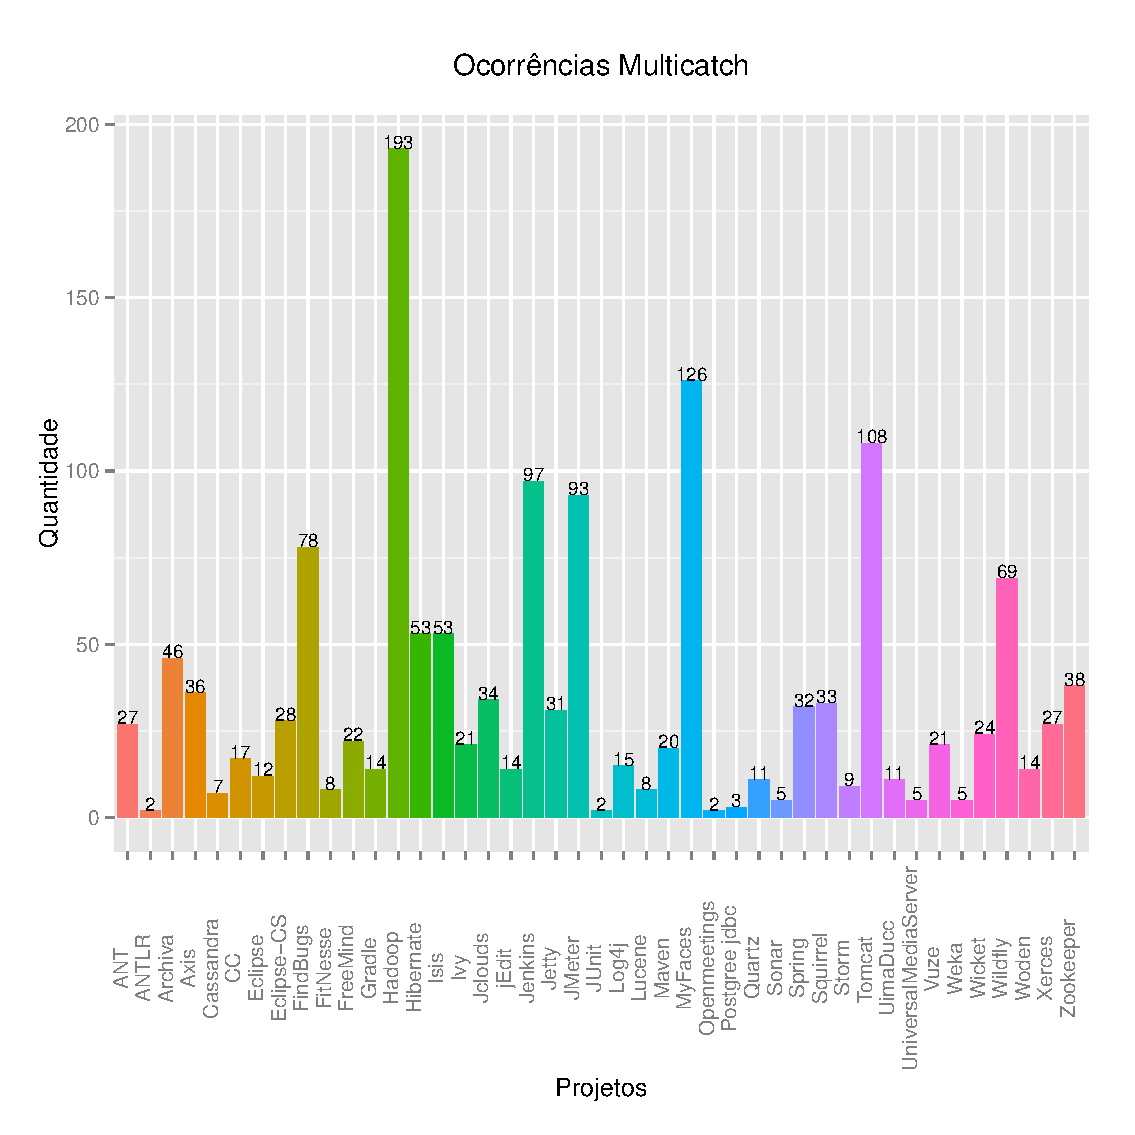
\includegraphics[width=1.0\textwidth]{Imagens/ocorrenciasMulticatch}
	\label{fig:Muticatch}
	\caption{Oportunidades de \textit{Multicatch} nos projetos.}
\end{figure}


De forma mais detalhada uma análise sobre uma classe do \textit{Spring 4.2.0.RC2} como exemplo é  \textit{org.springframework.beans.AbstractNestablePropertyAccessor.java}, o qual é possível verificar que tal característica é simples e rápida de ser implantada o que impacta em uma redução significativa do trecho de código mencionado algo entorno de 58\%.\\
\begin{lstlisting}
	// Sem uso de Multicacth 17LOC
	try {
		return this.typeConverterDelegate.convertIfNecessary(propertyName, oldValue, newValue, requiredType, td);
	}catch (ConverterNotFoundException ex) {
		PropertyChangeEvent pce =
			new PropertyChangeEvent(this.rootObject, this.nestedPath + propertyName, oldValue, newValue);
		throw new ConversionNotSupportedException(pce, td.getType(), ex);
	}catch (ConversionException ex) {
		PropertyChangeEvent pce =
			new PropertyChangeEvent(this.rootObject, this.nestedPath + propertyName, oldValue, newValue);
		throw new TypeMismatchException(pce, requiredType, ex);
	}catch (IllegalStateException ex) {
		PropertyChangeEvent pce =
			new PropertyChangeEvent(this.rootObject, this.nestedPath + propertyName, oldValue, newValue);
		throw new ConversionNotSupportedException(pce, requiredType, ex);
	}catch (IllegalArgumentException ex) {
		PropertyChangeEvent pce =
			new PropertyChangeEvent(this.rootObject, this.nestedPath + propertyName, oldValue, newValue);
		throw new TypeMismatchException(pce, requiredType, ex);
	}
	
// Com uso de Multicatch 10LOC
	try {
		return this.typeConverterDelegate.convertIfNecessary(propertyName, oldValue, newValue, requiredType, td);
	}catch (ConverterNotFoundException ex | IllegalStateException ex | ConversionException ex | IllegalArgumentException ex) {
		PropertyChangeEvent pce = 
			new PropertyChangeEvent(this.rootObject, this.nestedPath + propertyName, oldValue, newValue);
		
		if(ex instanceof ConversionException || ex instanceof IllegalArgumentException){
			throw new TypeMismatchException(pce, requiredType, ex);
		}else{
			throw new ConversionNotSupportedException(pce, td.getType(), ex);
		}
	}	
\end{lstlisting}
 

Uma análise mais detalhada sobre \textit{Spring} com 2620 ocorrências o que resulta em  afima que tal procedimento de tratar exceções estão presentes em todas as versões analisadas, iniciando na 3.0.0.M1 lançada em junho de 2009 até a mais recente até o momento 4.2.0.RC2. Para uma análise mais criteriosa será elaborada um detalhamento a partir da versão 4.0.0.M1 até a 4.2.0.RC2 totalizando 927 oportunidades de \textit{multicatch} 35\% das ocorrências no \textit{Spring}.\\

Conforme exibido na figura: \ref{fig:ocorrenciasMulticatchSpring}, obtem-se antes de um \textit{refactoring} uma média de 371 \acs{LOC} e após uma proposta concisa de \textit{refactoring} é possível obter uma média de 106 \acs{LOC} o que proporciona uma redução significativa de 71,46\%.\\

% a possibilidade de que após a criação das classes estes trechos não sofram um significativo \textit{refactoring} e nem uma evolução para essa característica citada o que pode acarretar em uma propagação de um estilo ultrapassado de programação na linguagem \textit{Java}.\\

\begin{figure}[h]
	\center
	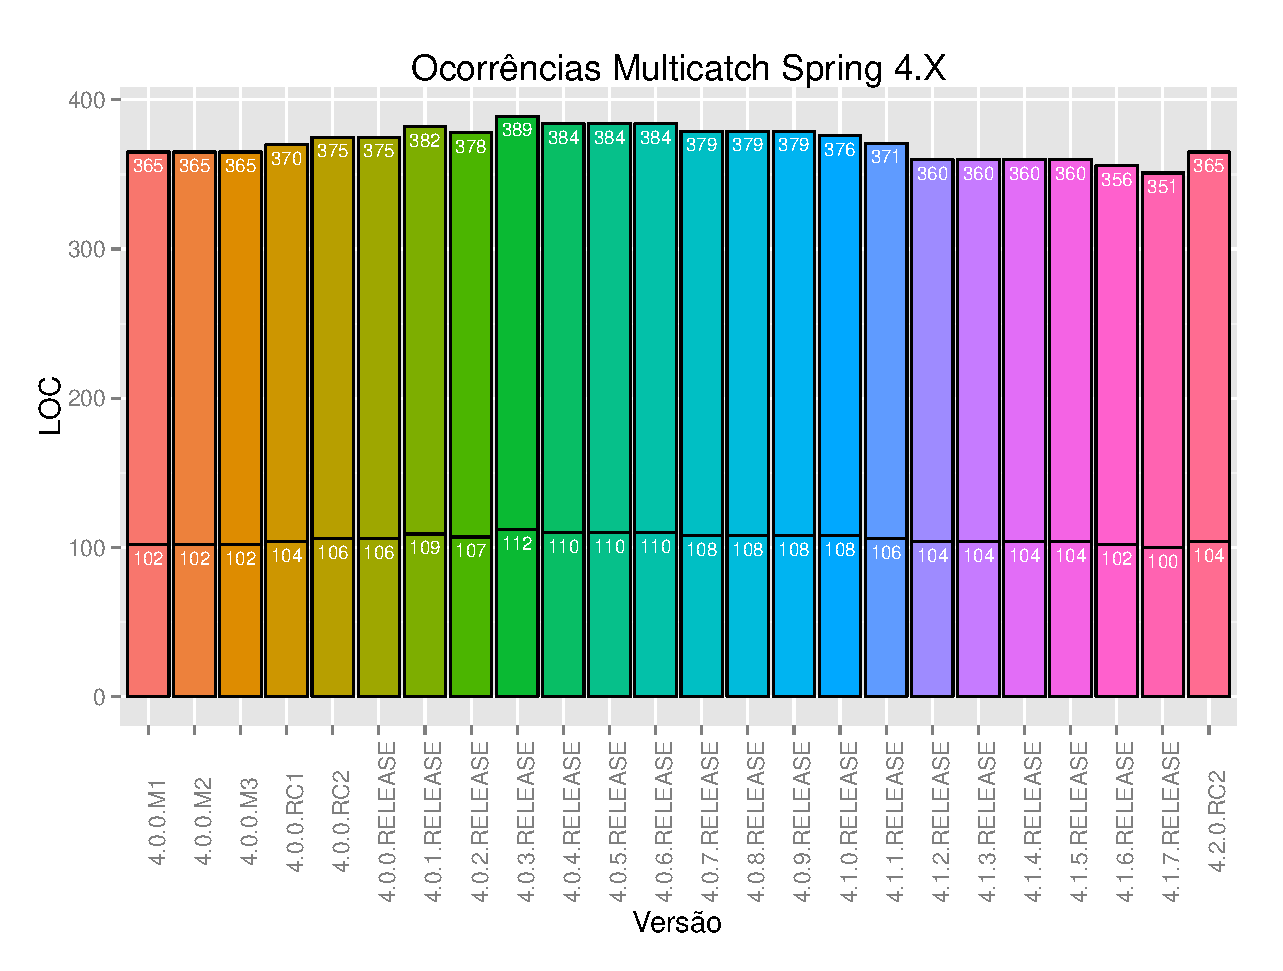
\includegraphics[width=1.0\textwidth]{Imagens/ocorrenciasMulticatchSpring}
	\label{fig:ocorrenciasMulticatchSpring}
	\caption{Ocorrências de \textit{Multicatch} Spring 4.X.}
\end{figure}


Dada uma redução significativa é impossível acreditar que projetos tão renomado não fazem uso desta \textit{feature}.  Ignorando uma característica que prove um código mais conciso e elegante conforme a proposta original desta \textit{feature} pela Oracle em 2007.\\


\section{ANT}
Até a última versão deste projeto \cite{apacheAnt}, 1.9.5, não foram encontradas utilização métodos com \textit{vargs}, expressões lambdas, \textit{switch} com \textit{strings} e nem \textit{try} com \textit{resources}.\\

Este projeto faz um bom uso de tratamento de exceções sendo encontrado em toda história de desenvolvimento foram produzidas 28 versões deste e com um total de 34722 blocos \textit{trys}, onde em média foram encontradas 1240 destes blocos por versão. E deste total pode-se verificar um total de 513 ocorrências de blocos \textit{trys} com \textit{catchs} iguais totalizando em 1,5\% de código repetido neste quesito conforme ilustra Figura: \ref{fig:TrysAnt}.\\

\begin{figure}[h]
	\center
	\includegraphics[width=0.7\textwidth]{Imagens/trysAnt}
	\label{fig:TrysAnt}
	\caption{Tratamento de exceção ao longo das releases.}
\end{figure}

Entretanto pode-se constatar conforme ilustrado na Figura: \ref{fig:catchIguais} que em todas as versões do projeto \textit{ANT} possui o tratamento de exceção como blocos \textit{catchs} iguais sendo contabilizado um total de 513 ocorrências e dando atenção especial entre as versões 1.9.0 e 1.9.5. Entretanto a partir da versão 1.9.0 por volta de 2012, java possuía o mecanismo de \textit{multicatch} que fora lançado por volta de 2011 em java 7. Entre as \textit{releases} desta versão foram encontradas em cada um dos 5 lançamentos do \textit{ANT} por volta de 27 ocorrências iguais de \textit{catchs} e acarreta em um total de 135 blocos repetidos. Caso fosse adotado \textit{multicatch} seria reduzido somente a 5 blocos a cada versão existente o que seria uma redução de código repetido em aproximadamente 18\%, e isso acarretaria em um código mais atual e elegante.\\

	\begin{figure}[h]
		\center
		\includegraphics[width=0.7\textwidth]{Imagens/catchsIguais}
		\label{fig:catchIguais}
		\caption{Bloco Try com catchs iguais ao longo das releases.}
	\end{figure}


Outro fato de bastente relevância é que o ANT faz uso de atributos parametrizados indicados na Figura: \ref{fig:atributosParametrizadosAnt}  e métodos parametrizados conforme Figura: \ref{fig:metodosParametrizadosAnt} desde sua versão 1.7.0, dezembro de 2006, o que leva a crer que foi aderido juntamente com o lançamento de \textit{Generics}, o que foi um marco na linguagem Java.\\

Vale ressaltar que de um total de 244137 atributos foi encontrado 1408 destes sendo paramentrizados o que acarreta em menos de 1\% dos atributos são genéricos. E a respeito dos métodos foram encontrados um total de 282216 métodos sendo que deste somente 1080 são métodos parametrizados acarretando em menos de 1\% são parametrizados.\\

O que leva a concluir que apesar do ANT fazer uso de tipos genéricos estes podem estar sendo subutilizados nesse projeto, ou esta característia não é de grande relevância para o projeto.\\



	\begin{figure}[h]
		\center
		\includegraphics[width=0.7\textwidth]{Imagens/atributosParametrizados.png}
		\label{fig:atributosParametrizadosAnt}
		\caption{Atributos parametrizados ao longo das releases.}
	\end{figure}
	
	
	\begin{figure}[h]
		\center
		\includegraphics[width=0.7\textwidth]{Imagens/metodosParametrizados.png}
		\label{fig:metodosParametrizadosAnt}
		\caption{Métodos parametrizados ao longo das releases.}
	\end{figure}

  
  \postextual
  \bibliographystyle{plain}
  \bibliography{referencias/referencias}
	
 % \printglossaries
\end{document}
